\documentclass{oci}
\usepackage[utf8]{inputenc}
\usepackage{lipsum}

\title{Rotar}
\codename{rotar}

\begin{document}
\begin{problemDescription}

  \centerline{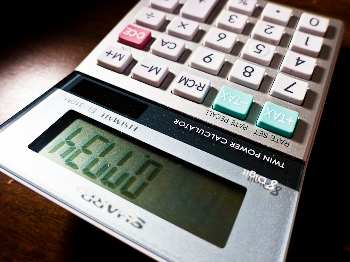
\includegraphics[scale=0.5]{upside-down.jpg}}

  Wax y Camilo, estudiantes del liceo OCI (Oportunidad para Cabros Inteligentes (?)), tienen prueba de química en un par de horas
  y evidentemente ayer no estudiaron nada.\\

  Pero todavía tienen una salvación, la prueba es con calculadora, y en lugar de utilizarla para sus cálculos,
  Wax y Camilo están decididos a usarla para hacer trampa. Para eso, le pasarán una calculadora a su amigo Jorgito, el mateo de la clase quién les dará las respuestas a través de la calculadora...\\

  Pero ¿cómo podrán hacerlo ? ¡La respuesta está en el techo! En el techo de la sala hay un espejo, y a través de él Wax y Camilo podrán ver la calculadora de Jorgito. \\

  \textit{Pero el espejo va a dar vuelta el número, y se verá rotado en 180 grados!} dice Camilo. Wax le dice que no se preocupe, que la mayoría de los números quedan iguales después de rotarlos en 180 grados. Como por ejemplo el 69 y el 25.\\

  Camilo no le cree, ya que hay números como el 12 o el 37 que al rotarlos en 180 grados cambian. Así deciden apostar un centella para ver quién tiene razón.\\

  Tu tarea es hacer un programa que reciba un número y verifique si al rotarlo en 180 grados queda igual o no.

\end{problemDescription}

\begin{inputDescription}
En la primera línea un entero \textbf{T} que representa el número de casos.
A continuación \textbf{T} líneas, cada uno contiene un único número entero \textbf{N}
\end{inputDescription}

\begin{outputDescription}
El output consiste en \textbf{T} líneas, cada una de las cuales debe tener la palabra \textit{Wax} si Wax tiene razón para el número correspondiente, y \textit{Camilo} si no.
\end{outputDescription}

\begin{scoreDescription}
  \score{6} $1 \le T \le 100, 0 \le N < 10$
  \score{6} $1 \le T \le 100, 0 \le N < 100$
  \score{6} $1 \le T \le 100, 0 \le N < 10^5$
  \score{6} $1 \le T \le 100, 0 \le N < 10^{10}$
  \score{6} $1 \le T \le 100, 0 \le N < 10^{10000}$
\end{scoreDescription}

\begin{sampleDescription}
\sampleIO{sample-1}
\sampleIO{sample-2}
\end{sampleDescription}

\end{document}
